\documentclass{article}

\usepackage[a4paper,left=3cm, top=3cm, right=3cm, bottom=3cm]{geometry}
\usepackage{amsmath}
\usepackage{amsfonts}
\usepackage{amsthm}
\usepackage{amssymb}
\usepackage{mathtools}
\usepackage[dvipsnames]{xcolor}
\usepackage{tikz}
\usepackage{subcaption}
\usepackage[linesnumbered,lined,boxed,commentsnumbered]{algorithm2e}
\usepackage{todonotes}
\usepackage[colorlinks=true, allcolors=blue]{hyperref}

\theoremstyle{plain}
\newtheorem{thm}{Theorem}
\newtheorem{lemma}{Lemma}
\newtheorem{claim}{Claim}[thm]
\newtheorem{observ}{Observation}[section]

\theoremstyle{definition}
\newtheorem{defn}{Definition}

\newcommand{\lca}{\mathrm{lca}}
\newcommand{\bigO}{\mathcal{O}}
\newcommand{\trios}{\mathcal{R}}
\newcommand{\quartets}{\mathcal{Q}}

\title{Solving MAF Using ILP With Trios and Quartets}
\author{}
\date{}

\begin{document}
  \maketitle

  \section{Preliminaries}

  By LCA we mean \emph{lowest common ancestor}. For now assume we have a rooted tree $T = (V,E)$, where
  $\rho$ denotes the root vertex. For two vertices $u, v \in V$ we say that $u < v$, $u$ \emph{lies below} $v$,
  if $v$ lies on the unique $\rho-u$ path.

  More precisely we define for any subset $S \subseteq V$ their lca as a vertex $v \in V$, for which
  $\forall s \in S: s \leq v$ and it is smallest one, i.e. no other such $u \in V, u < v$ exsits.
  We denote this as $\lca(S)$. When we talk about sets of specific elements, for example
  $S = \{u,v\}$ then we abreviate our notation to $\lca(a,b)$ only.

  Let us denote the trees on input as $\mathcal{T} = \{T_1, T_2, \dots, T_t\}$. Each tree has set $X$
  as its leafs of size $|X| = n$. Now the goal is to find an agreement forest
  $\mathcal{F} = \{F_1, F_2, \dots, F_r\}$ for minimum value of $r$.

  \section{Integer Linear Program}

  We use the ILP defined by Wu \cite{wuPracticalMethodExact2009}. We reuse the notation of \emph{trios} from
  \cite{ilp-maf}, because they use similar constraints, and also add the term \emph{quartets}.

  We use the following notation for tree $T$ and set $Y \subseteq X$. We define
  $T[Y]$ to be the smallest subtree of $T$ having all leafs $Y$.
  Next, $T|_Y$ stands for $T[Y]$ with forced contractions.

  To speed up the implementation we use LCA to classify all cases
  in a constant time if we precompute the LCA table for all pairs of nodes.

  We look at trios denoted as $a,b|c$ such that it looks like on the picture \ref{fig:trio}.
  Observe that this is the only constelation in which three leafs $R = \{a,b,c\}$ can encounter
  in $T|_R$, unless the labels are switched. Also see that $a,b|c$ and $b,a|c$ has the
  same properties hence we do not distinquish them.

  Next look at quartets, here we have more options because we only care if the paths intersect or not.
  We will denote them as $a,b|c,d$. We may see two examples of such occurance on Figure \ref{fig:quartet-fork} and Figure \ref{fig:quartet-line}.

  \begin{figure}[!ht]\centering
    \begin{subfigure}{.3\textwidth}\centering
      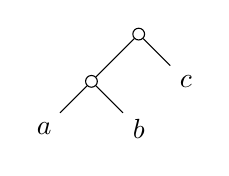
\begin{tikzpicture}[main/.style = {draw, circle, inner sep=1.5pt}, scale =.6]
        \node[main] (root) at (4,5) {};
        \node[main] (mid) at (3,4) {};
        \node (a) at (2,3) {$a$};
        \node (b) at (4,3) {$b$};
        \node (c) at (5,4) {$c$};
        \draw (root) -- (c);
        \draw (root) -- (mid);
        \draw (mid) -- (a);
        \draw (mid) -- (b);
      \end{tikzpicture}
      \caption{Trio.}\label{fig:trio}
    \end{subfigure}
    \begin{subfigure}{.3\textwidth}\centering
      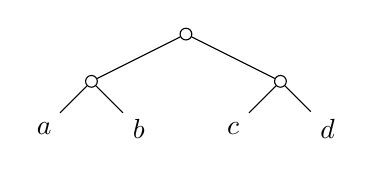
\begin{tikzpicture}[main/.style = {draw, circle, inner sep=1.5pt}, scale =.6]
        \node[main] (root) at (5,5) {};
        \node[main] (mid) at (3,4) {};
        \node[main] (mid2) at (7,4) {};
        \node (a) at (2,3) {$a$};
        \node (b) at (4,3) {$b$};
        \node (c) at (6,3) {$c$};
        \node (d) at (8,3) {$d$};
        \draw (root) -- (mid2);
        \draw (root) -- (mid);
        \draw (mid) -- (a);
        \draw (mid) -- (b);
        \draw (mid2) -- (c);
        \draw (mid2) -- (d);
      \end{tikzpicture}
      \caption{Quartet with incomparable LCAs.}\label{fig:quartet-fork}
    \end{subfigure}
    \begin{subfigure}{.3\textwidth}\centering
      \begin{tikzpicture}[main/.style = {draw, circle, inner sep=1.5pt}, scale =.6]
        \node[main] (root) at (4,5) {};
        \node[main] (mid) at (3,4) {};
        \node[main] (mid2) at (2,3) {};
        \node (c) at (4,3) {$c$};
        \node (d) at (5,4) {$d$};
        \node (a) at (1,2) {$a$};
        \node (b) at (3,2) {$b$};
        \draw (root) -- (d);
        \draw (root) -- (mid);
        \draw (mid) -- (c);
        \draw (mid) -- (mid2);
        \draw (mid2) -- (a);
        \draw (mid2) -- (b);
      \end{tikzpicture}
      \caption{Quartet with comparable LCAs.}\label{fig:quartet-line}
    \end{subfigure}
  \end{figure}

  \subsection{Incompatible Trios}

  An incompatible trio is if in $T_1$ we have $a,b|c$ trio and in some $T_j$, for $1 < j \leq t$
  we have either $a,c|b$ or $b,c|a$. See that cutting one of the edges in $T_1[\{a,b,c\}]$ is enough
  to resolve this incompatible trio. This is due to the fact that one edge will
  remove one of $a,b$ or $c$ from the rest. Then the trio on itself would be fine
  with the definition of MAF. 

  It is easy to find such occurance of incompatible trios in our input. First, we go
  over all triples of leafs $a,b,c$, in $\bigO(n^3)$ time, and find such triple that
  suffices the following inequality. $\lca_1(a,b) \neq \lca_1(a,b,c)$. Since
  easily seen it must be $\lca_1(a,b) \leq \lca_1(a,b,c)$, then when inequality
  occurs it is our trio. Then, we go through all other trees and if
  there is trio for which $\lca_j(a,b) = \lca_j(a,b,c)$ we have found incompatible
  trio.

  So we gather all trios into the set of $\trios$ and we define $\mathcal{L}(R)$
  to be $T_1[R]$, for $R \in \trios$.

  \subsection{Incompatible Quartets}

  Now, we look at quartest. It is a bit harder to find such quartet by using LCAs only. The
  definition is based on the intersection of $a-b$ and $c-d$ paths.

  Firstly, it must be true that $\lca_1(a,b) \neq \lca_2(c,d)$. Otherwise their paths intersect.
  Next we split into two cases.

  \begin{enumerate}
    \item First, if $\lca_1(a,b,c) = \lca_1(a,b)$ then we check that $\lca_1(c,d)$ is not the same
      as $\lca_1(x,y)$ for $x \in \{a,b\}$ and $y \in \{c,d\}$.
    \item Second, that the equality does not hold. Then we check that $\lca_1(a,b)$ is not the
      same as $\lca_1(x,y)$ for $x,y$ same as before.
  \end{enumerate}

  Proof sketch. The very first check is clear. Next in the first branch we get that $c$ is below $a,b$ tree
  and then $d$ must be also below $a,b$ tree and then the further checks satsify this condition. In the
  other case we have that $a$ is below $c,d$ tree or they are completely disjoint. In the former
  case it is enough to check the values and in the latter case we actually do not need any further
  checks.

  Therefore we find quartets that satisfy this for the first tree and whenever we find a different tree
  for which this does not hold we say it is incompatible quartet.
  We collect all such quartets into $\quartets$ and for each $Q \in \quartets$ we
  define $\mathcal{L}(Q)$ as $T[\{a,b\}] \cup T[\{c,d\}]$.

  By using these definitions we create our ILP. And from \cite{wuPracticalMethodExact2009} we get
  that the optimal integer solution is actually a Maximum Agreement Forest as desired.

  \begin{align*}
    \text{Minimize: } & \sum_{e \in E(T_1)} x_e \\
    \text{Subject to: } & \sum_{e \in \mathcal{L}(R)} x_e \geq 1 & \forall R \in \trios \\
                & \sum_{e \in \mathcal{L}(Q)} x_e \geq 1 & \forall Q \in \quartets \\
            & x_e \in \{0, 1\} & \forall e \in E(T_1)
  \end{align*}

  \section{Reductions and Speed-Ups}

  We implement simple and known reduction to reduce the size of the input trees.
  We call $a,b \in X$ a \emph{cherry} (fig. \ref{fig:cherry}) if
  it $a$ and $b$ shares the same parent and this is in every tree from the input. Then we can reduce this
  by substituting their parent with $a$ and remember that $b$ is also included. Notably one
  cherry could lead to creating another cherry. But this can be done in linear time.

  \begin{figure}[!ht]\centering
      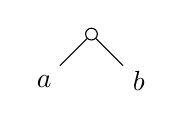
\begin{tikzpicture}[main/.style = {draw, circle, inner sep=1.5pt}, scale =.6]
        \node[main] (root) at (4,5) {};
        \node (a) at (3,4) {$a$};
        \node (b) at (5,4) {$b$};
        \draw (root) -- (a);
        \draw (root) -- (b);
      \end{tikzpicture}
      \caption{A cherry.}\label{fig:cherry}
  \end{figure}

  Moreover, we add additional constraints to help the ILP solver to solve it faster. We add two types of
  constraints. One is called \emph{fork} and the other \emph{extended fork}, see Figure \ref{fig:fork} and Figure \ref{fig:extended-fork}
  respectively. For fork we first observe that deleting two edges is always enough because the third is implicitly contracted.
  Moreover it is safe to say that if we remove exactly two edges then it is always the bottom two. In ILP formulation we may say
  that $2a + b + c \leq 2$. In the similar fashion we also introduce an extended fork, where we add constraint saying that
  $2a + 2b + 2c + d + e + f + g \leq 4$.

  \begin{figure}[!ht]\centering
    \begin{subfigure}{.45\textwidth}\centering
      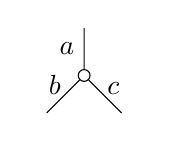
\begin{tikzpicture}[main/.style = {draw, circle, inner sep=1.5pt}, scale =.6]
        \node[main] (root) at (4,5) {};
        \node (a) at (3,4) {};
        \node (b) at (5,4) {};
        \draw (root) -- (a) node[near end, left, above] {$b$};
        \draw (root) -- (b) node[near end, right, above] {$c$};
        \draw (4,6) -- (root) node[midway, left] {$a$};
      \end{tikzpicture}
      \caption{A simple fork.}\label{fig:fork}
    \end{subfigure}
    \begin{subfigure}{.45\textwidth}\centering
      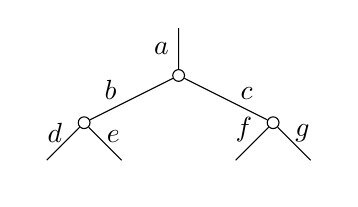
\begin{tikzpicture}[main/.style = {draw, circle, inner sep=1.5pt}, scale =.6]
        \node[main] (root) at (4,5) {};
        \node[main] (a) at (2,4) {};
        \node[main] (b) at (6,4) {};
        \draw (root) -- (a) node[near end, left, above] {$b$};
        \draw (root) -- (b) node[near end, right, above] {$c$};
        \draw (4,6) -- (root) node[midway, left] {$a$};
        \node (c) at (1,3) {};
        \node (d) at (3,3) {};
        \node (e) at (5,3) {};
        \node (f) at (7,3) {};
        \draw (a) -- (c) node[near end, left, above] {$d$};
        \draw (a) -- (d) node[near end, right, above] {$e$};
        \draw (b) -- (e) node[near end, left, above] {$f$};
        \draw (b) -- (f) node[near end, right, above] {$g$};
      \end{tikzpicture}
      \caption{An extended fork.}\label{fig:extended-fork}
    \end{subfigure}
  \end{figure}

  Another very straigthforward constraint is that the sum of all edges in $T_1$ is at most $n-2$. That is
  due to the fact that there is always a simple solution where every tree in MAF is a node except for
  one simple two-leaf tree. Moreover, we can have a lower bound for this as well if we have some, possibly
  infeasible, MAF.

  We have added at most $\O(n)$ additional constraints, which is not much. On the other hand we can have
  upto $\O(n^3 + n^4)$ constraints for trios and quartets, which is still polynomial, but not really nice.
  As it turns out it is rarely the case. But we can still do better by choosing only some constraints
  and then iteratively add new ones and solve the new ILP. Therefore we sort all trios and quartets based
  the number of edges in it in an increasing way. Then we choose all constraints which are of length
  at most $2 \log_2(n)$. If there is not enough of them then we always add at least $n$ constraints.
  In the next iterations we always have some forrest and possibly unsatisfied constraints. We go through
  all the constraints and if (1) there is no unsatisfied constraint then we are done, otherwise (2) we
  add at most $n$ new constraints of each type, i.e., trios and qaurtets. This serves as a lower bound
  for the very last constraint summing all edges.

  \bibliographystyle{alpha}
  \bibliography{ref}
\end{document}
